\documentclass[10pt,a4paper]{book}
\usepackage[utf8]{inputenc}
\usepackage{amsmath}
\usepackage{amsfonts}
\usepackage{amssymb}
\usepackage{wasysym}
\usepackage{multicol}
\usepackage{hyperref}
\usepackage{tabularx}
\usepackage{subfig}
\usepackage{tikz}
\usepackage[ruled, lined, longend]{algorithm2e}
\usepackage[shortlabels]{enumitem}
\usepackage{textcomp}
\usepackage{chemfig}

\setlength{\parindent}{20pt}
\hypersetup{
    colorlinks,
    citecolor=black,
    filecolor=black,
    linkcolor=black,
    urlcolor=darkgray
}

\newcommand{\R}{\mathbb{R}}
\newcommand{\N}{\mathbb{N}}
\newcommand{\Z}{\mathbb{Z}}
\newcommand{\x}{$\times$ }
\newcommand{\ind}{\hspace*{\parindent}}

\title{Algèbre linéaire \vspace{0.2cm} - Résumé}
\author{Mahel Coquaz}
\date{Semestre de printemps 2025}

\begin{document}
\maketitle
\tableofcontents
\newpage
%\part*{Atomistique}
\section*{Introduction}
Ce qui suit se veut être un résumé du cours d'Algèbre pour MàN (PREPA-032) donné au semestre de printemps 2025 à l'EPFL. Le contenu de ce cours ne m'appartient pas et est quasiment intégralement extrait du cours des Professeurs Mathieu Huruguen, Simon Bossoney et Sacha Friedli qui l'ont enseigné. J'ai cependant modifié des formulations et ajouté des notes lorsqu'il me semblait pertinent de le faire. \par
Ce résumé/polycopié n'est pas exempt d'erreurs, si vous en trouvez une, vous pouvez me contacter sur mon adresse EPFL \texttt{\href{mailto:mahel.coquaz@epfl.ch}{mahel.coquaz@epfl.ch}} ou via le repo GitHub \url{https://github.com/hotwraith/LectureNotes}. \par
Le repository GitHub est aussi où se trouvent les dernières versions des fichiers PDFs et \TeX pour ce cours (et éventuellement d'autres). \par
Enfin (et surtout) l'algèbre linéaire est une matière où la visualisation des concepts peut permettre d'avoir une bien meilleure intuition, comme ce résumé se concentre sur l'aspect calculatoire je ne peux que vous recommander de visionner les vidéos 
\textbf{\href{https://youtube.com/playlist?list=PLZHQObOWTQDPD3MizzM2xVFitgF8hE_ab}{Essence of linear algebra}} de 3Blue1Brown pour vous faire une meilleure intuition des concepts abordés.

\subsection*{Notations}
Dans ce résumé les notations suivantes seront utilisées sauf mention du contraire:
\begin{itemize}
\item Les matrices seront dénotées par une lettre majuscule (A, B, C, ...)
\item Les éléments de ces matrices seront dénotés par une lettre grecque avec ij la ligne et colonne de position de l'élément (\(\alpha_{ij}, \beta_{ij}, \gamma_{ij}\), ...)
\item rg(A) = rang de la matrice A. dim(A) = dimension de la matrice A. det(A) = déterminant de la matrice A.
\item Les constantes quelconques appartenant à $\R$ seront \textbf{en général} dénotées par $\lambda$ ou k.
\item $\hat{i}$ et $\hat{j}$ sont les vecteurs unitaires de la base canonique, \(\hat{i} = \left(\begin{array}{c} 1 \\ 0 \end{array}\right)\), \(\hat{j} = \left(\begin{array}{c} 0 \\ 1 \end{array}\right)\) (pour $\R^2$)
\item On note $\vec{v}$ un vecteur quelconque exprimé en base canonique et $[\vec{v}]_B$ le même vecteur exprimé en coordonées de la base B.
\item On note $\mathbb{B}$ la base canonique et \textbf{B} une base autre quelconque. 
\end{itemize}

\chapter{Calcul matriciel}

\section{Opérations matricielles}

\paragraph{Définition d'une matrice} Une matrice est un tableau de taille \textbf{n \x p}\footnote{On utilise aussi \textbf{m \x n} dans certaines notations.} avec n le nombre de \textbf{lignes} et p le nombre de \textbf{colonnes}. \\
Exemple avec n = p = 2:
\[\begin{pmatrix}
a & b \\
c & d
\end{pmatrix}\] \\
On dénote un élément quelconque position de la matrice par $\alpha_{ij}$ avec \textbf{i sa ligne} et \textbf{j sa colonne}. Exemple: a est l'élément $\mathbf{\alpha_{11}}$ et b l'élément $\mathbf{\alpha_{12}}$.

\subsection{Addition de matrices}

Soit deux matrices A et B de \textbf{même taille} n \x p. 
\[
\begin{pmatrix}
a & b \\
c & d
\end{pmatrix}
+
\begin{pmatrix}
a' & b' \\
c' & d'
\end{pmatrix}
=
\begin{pmatrix}
a + a' & b + b' \\
c + c' & d + d'
\end{pmatrix}
\]
Formant une nouvelle matrice C composés d'éléments $\gamma_{ij}$. \par
Soit pour tout élément $\gamma_{ij} \in$ C, la nouvelle matrice on a:
\[\gamma_{ij} = \alpha_{ij} + \beta_{ij}\]

\subsection{Multiplication scalaire}

Soit une matrice A d'éléments $\alpha_{ij}$ et un scalaire $\lambda \in \R$ et C notre matrice de résultat composés des éléments $\gamma_{ij}$.
\[\lambda A = C\]
\[\lambda
\begin{pmatrix}
a & b \\
c & d
\end{pmatrix}
=
\begin{pmatrix}
\lambda a & \lambda b \\
\lambda c & \lambda d 
\end{pmatrix}\]
Soit tous les éléments $\in$ C:
\[\gamma_{ij} = \lambda \times \alpha_{ij}\]

\subsection{Produit matriciel}
Soit trois matrices A, B et C respectivement composées des éléments $\alpha_{ij}$, $\beta_{ij}$, $\gamma_{ij}$, on a:
\[A \cdot B = C\]
\[\begin{pmatrix}
a & b \\
c & d
\end{pmatrix}
\cdot
\begin{pmatrix}
a' & b' \\
c' & d'
\end{pmatrix}
=
\begin{pmatrix}
aa' + bc'  & ab' + bd' \\
ca' + dc' & cb' + dd'
\end{pmatrix}\]
On note qu'il faut que A, de taille m \x n, et B de taille n \x p pour que la multiplication soit possible (avec m et p $\in \R$)
Ou de manière générale:
\[\gamma_{ij} = \sum_{k=1}^n \alpha_{ik} \beta_{kj}\]
et on obtient une matrice C de taille \textbf{m \x p}.

\subsection{Propriétés}

\begin{itemize}
\item A + B = B + A (commutativité)
\item A + (B + C) = (A + B) + C (associativité)
\item A $\cdot$ (B + C) = A $\cdot$ B + A $\cdot$ C (distributivité)
\item A $\cdot$ (B $\cdot$ C) = (A $\cdot$ B) $\cdot$ C
\end{itemize}

\section{Opérations et matrices élémentaires}

\subsection{Opérations élémentaires}

Soit A une matrice de taille n \x p, d'éléments $\alpha_{ij}$, de colonnes $C_i$ et de lignes $L_j$.
\paragraph{Sur les lignes $L_j$}
\begin{itemize}
\item $L_j \leftrightarrow L_k$ ($j \neq k$)
\item $L_j \leftarrow \lambda L_j$ ($\lambda \neq 0$)
\item $L_j \leftarrow L_j + \lambda L_k$ ($\lambda \in \R$, $j \neq k$)
\end{itemize}
Ces opérations ne changent \textbf{pas} l'ensemble de solutions de A$\vec{x}$ = $\vec{b}$. Elles sont dites \textbf{inversibles}.

\paragraph{Sur les colonnes $C_i$}
\begin{itemize}
\item $C_i \leftrightarrow C_k$ ($j \neq k$)
\item $C_i \leftarrow \lambda C_i$ ($\lambda \neq 0$)
\item $C_i \leftarrow C_i + \lambda C_k$ ($\lambda \in \R$, $j \neq k$)
\end{itemize}

Ces \textbf{opérations élémentaires} sont la base de la méthode de Gauss pour résoudre des systèmes linéaires: \textbf{l'échelonnement}.

\section{Rang, déterminant et décomposition colonne-ligne}

\subsection{Rang}
Lors d'une application linéaire représentée par une matrice A on appelle \textbf{rang(A) = dim(Im(A))}. \par
Le rang de A (ou sa dimension image) représente l'ensemble des possibilités après une application linéaire. Il est représenté par le \textbf{nombre de pivots} restants après l'échelonnement d'une matrice. \\
Un exemple: \\
On prend A de taille 2 \x 2 et de rg(A) = 2. Pour un $\vec{x}$ quelconque A$\vec{x}$ sera représenté sur un plan de dimension 2. \par
Une application linéaire représente une transformation de l'espace d'origine vers un nouvel espace. Celui ci peut-être au mieu de même dimension que la matrice d'origine, au pire de rang 0 (l'espace se contracte en un point: l'origine (0, 0)). \\
Exemple avec rg(A) = 1:
\[A \cdot I_2 = ?\]
\[\begin{pmatrix}
1 & 2 \\
2 & 4
\end{pmatrix}
\cdot
\begin{pmatrix}
1 & 0 \\
0 & 1
\end{pmatrix}
=
\begin{pmatrix}
1 & 2 \\
2 & 4
\end{pmatrix}
\]
Ici les colonnes des la matrice $I_2$ représentent les vecteurs de la base canonique $\hat{i}$ et $\hat{j}$ auxquels on applique l'application linéaire A. \\
On remarque qu'après coup $\hat{i}$ = \(\left(\begin{array}{c} 1 \\ 2 \end{array}\right)\) et $\hat{j}$ = \(\lambda \hat{i}\) avec $\lambda = 2$. Par conséquent l'ensemble représentable est devenu une ligne et non plus un plan ($\R_2 \rightarrow \R_1$).

\subsection{Déterminant}

\paragraph{Propriétés}
\begin{itemize}
\item Le déterminant n'est pas affecté par les opération élémentaires sur les lignes/colonnes. 
\item Multiplier une ligne de la matrice A par $\lambda \in \R \rightarrow \lambda \cdot det(A)$ 
\item Échanger deux lignes ou deux colonnes (\(L_i \leftrightarrow L_k\) ou \(C_i \leftrightarrow C_k\)) revient à changer le signe du déterminant.
\item Le déterminant $det(A)$ représente dans $\R_2$ la multiplication de l'aire causée par l'application linéaire A, et dans $\R_3$ la multiplication du volume.
\item $det(AB) = det(A) \cdot det(B)$
\item Si $det(A) \neq 0$ alors A possède une matrice inverse $A^{-1}$ qui satisfait $AA^{-1} = A^{-1}A = I_n$ 
\end{itemize}

\paragraph{Déterminant d'une matrice 2 \x 2} Le déterminant d'une matrice 2 \x 2 s'écrit de la manière suivante: 
\[det\left(\begin{pmatrix}
a & b \\
c & d
\end{pmatrix}\right)
= ad - bc
\]
Note de lecture:
\begin{itemize}
\item det(A) = 0 $\Longleftrightarrow$ rg(A) $\leq$ 1 
\item det(A) $\neq$ 0 $\Longleftrightarrow$ rg(A) = 2 
\end{itemize}
Comme nous sommes dans $\R_2$ un déterminant = 0 signifie que tous les points de notre espace ont été "écrasés" sur une ligne ($\R_1$) ou un point (l'origine), donc l'aire du parallépipède formés par les vecteurs d'une matrice quelconque est forcément nulle (vecteurs colinéaires). Si on a encore une aire après l'application linéaire alors notre rg(A) = 2 car on peut encore former un parallépipède.


\paragraph{Déterminant d'une matrice 3 \x 3}
\[det(A)= det\left( 
\begin{pmatrix}
 a & b & c \\
 d & e & f \\
 g & h & i
\end{pmatrix}\right)\]
\[\Rightarrow det(A) = a\cdot det\left(\begin{pmatrix}
e & f \\
h & i
\end{pmatrix}\right)
-b\cdot det\left(\begin{pmatrix}
d & f \\
g & i
\end{pmatrix}\right)
+c\cdot det\left(\begin{pmatrix}
d & e \\
g & h
\end{pmatrix}\right)\]
\[\Rightarrow det(A) = a\cdot (ei-fh) - b \cdot (di - fg) + c \cdot (dh -eg)\]\\
\footnote{Développement par colonnes.}
ou
\[\Rightarrow det(A) = a\cdot det\left(\begin{pmatrix}
e & f \\
h & i
\end{pmatrix}\right)
-d\cdot det\left(\begin{pmatrix}
b & c \\
h & i
\end{pmatrix}\right)
+g\cdot det\left(\begin{pmatrix}
b & c \\
e & f
\end{pmatrix}\right)\]
\[\Rightarrow det(A) = a\cdot (ei-fh) - d \cdot (bi - ch) + g \cdot (bf - ce)\]\footnote{Développement par lignes.}
Le signe du coefficient est déterminé par la logique suivante:
\[\begin{pmatrix}
+ & - & + \\
- & + & - \\
+ & - & +
\end{pmatrix}\]

\subsection{Décomposition colonne ligne}
%TODO méthode généraliste
Exemple pour une matrice 2x2:
\[\begin{pmatrix}
2 & 4 \\
3 & 6
\end{pmatrix}
= \left\lbrace \begin{array}{rcl}
2x & + & 4y \\
3 x & + & 6y
\end{array} \right.
\]
\[\Rightarrow \left\lbrace \begin{array}{rcl}
2 & (x + 2y) \\
3 & (x + 2y)
\end{array} \right.
\Rightarrow
\begin{pmatrix}
2 \\ 3
\end{pmatrix}
\begin{pmatrix}
1 & 2
\end{pmatrix}
\]

\section{Inverses}
Un inverse existe pour une matrice A quelconque n'existe que pour $det(A) \neq 0$, la logique ? Si la matrice d'application linéaire A n'est pas de rg(A) = dim(A) alors il n'est pas possible pour elle de faire $\R_n \rightarrow \R_{n-1} \rightarrow \R_n$ telle que $AA^{-1} = A^{-1}A = I_n$.

\subsection{Inverses 2 \x 2}

\[A = \begin{pmatrix}
a & b \\
c & d
\end{pmatrix}
\]
\[A^{-1} = \frac{1}{det(A)} \begin{pmatrix}
\mathbf{d} & \textcolor{green}{-b} \\
\textcolor{green}{-c} & \mathbf{a}
\end{pmatrix}
\]

\subsection{Inverses 3 \x 3}

On échelonne réduit A face à $I_3$ en répétant chaque opération élémentaire faites pour réduire A sur $I_3$
\[A | I_3 \]
Exemple:
\[\left(\begin{array}{ccc|ccc}
1 & 2 & 0 & 1 & 0 & 0 \\
0 & 4 & 1 & 0 & 1 & 0 \\
-1 & 2 & 2 & 0 & 0 & 1
\end{array}
\right)\]
\[\Rightarrow \left(\begin{array}{ccc|ccc}
1 & 2 & 0 & 1 & 0 & 0 \\
0 & 4 & 1 & 0 & 1 & 0 \\
0 & 4 & 2 & 1 & 0 & 1
\end{array}
\right)\]
\[\Rightarrow \left(\begin{array}{ccc|ccc}
1 & 2 & 0 & 1 & 0 & 0 \\
0 & 4 & 1 & 0 & 1 & 0 \\
0 & 0 & 1 & 1 & -1 & 1
\end{array}
\right)\]
\[\Rightarrow \left(\begin{array}{ccc|ccc}
1 & 2 & 0 & 1 & 0 & 0 \\
0 & 4 & 0 & -1 & 2 & -1 \\
0 & 0 & 1 & 1 & -1 & 1
\end{array}
\right)\]
\[\Rightarrow \left(\begin{array}{ccc|ccc}
1 & 2 & 0 & 1 & 0 & 0 \\
0 & 1 & 0 & -\frac{1}{4} & \frac{1}{2} & -\frac{1}{4} \\
0 & 0 & 1 & 1 & -1 & 1
\end{array}
\right)\]
\[\Rightarrow \left(\begin{array}{ccc|ccc}
1 & 0 & 0 & \frac{3}{2} & -1 & \frac{1}{2} \\
0 & 1 & 0 & -\frac{1}{4} & \frac{1}{2} & -\frac{1}{4} \\
0 & 0 & 1 & 1 & -1 & 1
\end{array}
\right)\]
Le côté droit est la matrice inversée $A^{-1}$.

\chapter{Structures vectorielles de \texorpdfstring{$\R^2$ et $\R^3$}{R2 et R3}}

\section{Bases de \texorpdfstring{$\R^2$ et $\R^3$}{R2 et R3}}

\subsection{\texorpdfstring{$\R^2$}{R2}}

Une base de $\R^2 $ nécessite deux vecteurs linéairement indépendants, donc non-colinéaires, on écrit alors:
\[B = vec\left(\vec{v_1}, \vec{v_2}\right)\]
La base canonique $\hat{i}$, $\hat{j}$ de $\R^2$ est représentée par la matrice \(\begin{pmatrix}
1 & 0 \\ 0 & 1 \end{pmatrix}\), et un exemple de matrice de base de $\R^2$ serait \(\begin{pmatrix}1 & 2 \\ 3 & 4\end{pmatrix}\), car $\vec{v_1}$ et $\vec{v_2}$ ne sont pas linéairement dépendants. \\
Si $\vec{v_1}$ et $\vec{v_2}$ forment une base \textbf{B} de $\R^2$ et $\vec{v} \in \R^2$ ce $\vec{v}$ peut se décomposer en éléments \(\vec{v} = t_1\vec{v_1} + t_2\vec{v_2}\). On a $[\vec{v}]_B = \begin{pmatrix} t_1 \\ t_2 \end{pmatrix}$. \\
Exemple:
\[B = \begin{pmatrix}1 & 2 \\ 3 & 4\end{pmatrix} B^{-1} = \begin{pmatrix}-2 & 1 \\ 3/2 & -1/2\end{pmatrix} \; et \; \vec{v} = \begin{pmatrix} 2 \\ 1 \end{pmatrix}\]
\[[\vec{v}]_B = \begin{pmatrix}-2 & 1 \\ 3/2 & -1/2\end{pmatrix}\begin{pmatrix} 2 \\ 1 \end{pmatrix} = \begin{pmatrix} -3 \\ \frac{5}{2} \end{pmatrix}\]
On vérifie:
\[\vec{v} = -3\cdot \begin{pmatrix}1 \\ 3\end{pmatrix} + \frac{5}{2}\cdot \begin{pmatrix} 2 \\ 4 \end{pmatrix} = \begin{pmatrix} -3+5 \\ -9+10 \end{pmatrix} = \begin{pmatrix} 2 \\ 1 \end{pmatrix}\]
De manière plus générale:
\[\mathbf{\vec{v} = B\cdot [\vec{v}]_B}\]
\[\mathbf{[\vec{v}]_B = B^{-1}\cdot \vec{v}}\]

\subsection{\texorpdfstring{$\R^3$}{R3}}

Même logique que pour $R^2$, ici la base canonique $\hat{i}$, $\hat{j}$, $\hat{k}$ est représentée par la matrice $\begin{pmatrix} 1 & 0 & 0 \\ 0 & 1 & 0 \\ 0 & 0 & 1\end{pmatrix}$.\\
La logique de changement de base est la même.

\subsubsection{Droites et plans dans $\R_3$}

Si la base B est de rg(B) = 1 on a une droite vectorielle dans $R^3$, tous les éléments peuvent êtres accédés par $t\cdot \vec{v}$ avec $\vec{v}$ le vecteur directeur de la droite.\par
Si la base B est de rg(B) = 2 (soit Vect($\vec{v_1}, \vec{v_2}$)) elle engendre un plan au sein de l'espace. \\
L'équation du plan s'écrit:
\[det\left(\begin{pmatrix}
x & \alpha_1 & \beta_1 \\
y & \alpha_2 & \beta_2 \\
z & \alpha_3 & \beta_3 \\
\end{pmatrix}\right) = 0\]
La logique derrière ? Tous les vecteurs expressibles par $\vec{v} = \begin{pmatrix} x \\ y \\ z \end{pmatrix}$ doivent, pour appartenir au plan engendré, être la combinaison linéaire $\vec{v} = t_1\vec{v_1} + t_2\vec{v_2}$ des deux vecteurs linéairement indépendants de la base. \par
Une autre manière d'exprimer cela est avec det(Vect($\vec{v}, \vec{v_1}, \vec{v_2}$)) = 0, car cela implique que rg(Vect($\vec{v}, \vec{v_1}, \vec{v_2}$)) $\leq$ 2, or comme on sait que $v_1$ et $v_2$ engendrent un plan alors rg = 2 si det = 0. %TODO reformulate, c'est confus

\paragraph{Intersection de deux plans vectoriels dans $\R^3$}
Soit deux plans V et V' respectivement définis par \(\left\lbrace \begin{array}{rcl}
ax + by + cz = 0 \\
a'x + b'y + c'z = 0
\end{array} \right.\). \\
Si (a, b, c) et (a', b', c') sont \textbf{proportionnels} alors V = V' et l'intersection s'exprime selon l'équation de l'un des deux plans. \\
Si (a, b, c) et (a', b', c') ne sont \textbf{pas} proportionnels, 
\[V\cap V' = Vect(\vec{v_{int}})\]
où
\[v_{int} = \begin{pmatrix} a \\ b \\ c \end{pmatrix} \times \begin{pmatrix} a' \\ b' \\ c' \end{pmatrix} = \begin{pmatrix} -cb' + bc' \\ ca' - ac' \\ -ba' + ab'\end{pmatrix}\]

\section{Sous-espaces affines}

\subsection{Droites affines de \texorpdfstring{$\R^2$}{R2}}

On appelle droite affine \textbf{contenant} $\vec{v_0}$ et \textbf{dirigée par} $\vec{v_1}$ la droite V telle que:
\[V:= \left\lbrace\ v_0 + tv_1 \;|\; t \in \R \right\rbrace \subset \R^2\]
avec $v_0$, $v_1$ $\in \R^2$ ($v_1 \neq$ (0, 0))
\begin{figure}[h!]
\begin{center}
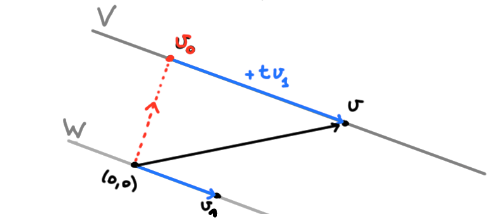
\includegraphics[scale=0.8]{./assets/schema_droites_affines.png}
\label{fig:droites_affines}
\caption{Exemple de droite affine}
\end{center}
\end{figure}
\\ Remarque: 
\begin{itemize}
\item Si $v_0$ = (0,0), V est une droite (et un espace) vectorielle.
\item Si $v_0$ $\neq$ (0,0), V n'est \textbf{pas} un espace vectoriel.
\item $v \in V$ $\Leftrightarrow$ $v-v_0 \in$ Vect($v_1$) $= W$
\item On a V le translaté de W par $v_0$:
\[V = v_0 + W = v_0 + Vect(v_1)\]
\item On appelle W la \textbf{droite vectorielle associée} à V.
\end{itemize}

\paragraph{Équation}
\[V: ax+by = c \tag*{Équation de la droite}\]
Il faut noter que $\vec{v_1} = \left( \begin{array}{c} -b \\ a \end{array} \right)$

\[W: ax+by= 0 \tag*{Équation de la droite vectorielle associée}\]

\subsection{Plans affines de \texorpdfstring{$\R^3$}{R3}}

\paragraph{Définition} Si $v_0, v_1, v_2 \in \R^3$ tels que $v_1, v_2$ non colinéaire, alors:
\[V:= \left\lbrace v_0 + t_1v_1 + t_2v_2 \;|\; t_1, t_2 \in \R \right\rbrace\ \subset \R^3 \]
\begin{itemize}
\item Si $v_0$ = (0,0,0), V est le plan et espace vectoriel.
\item Si $v_0 \neq$ (0,0,0), V est le plan affine \textbf{contenant} $v_0$ \textbf{dirigé par} $v_1$ et $v_2$
\item V = $v_0$ + Vect($v_1$, $v_2$) 
\item W = Vect($v_1$, $v_2$) est le \textbf{plan vectoriel associé à V}, ils sont \textbf{parallèles}.
\end{itemize}

\paragraph{Équation}
On prend $v_0 = \begin{pmatrix} x_0 \\ y_0 \\ z_0 \end{pmatrix}$, $v_1 = \begin{pmatrix} \alpha_1 \\ \alpha_2 \\ \alpha_3 \end{pmatrix}$, $v_1 = \begin{pmatrix} \beta_1 \\ \beta_2 \\ \beta_3 \end{pmatrix}$ et un $\vec{v} = \begin{pmatrix} x \\ y \\ z \end{pmatrix}$ on pose:
\[\begin{pmatrix}
x - x_0 & \alpha_1 & \beta_1 \\
y - y_0 & \alpha_2 & \beta_2 \\
z - z_0 & \alpha_3 & \beta_3
\end{pmatrix} = 0
\]
\[\Rightarrow ax+by+cz = ax_0+by_0+cz_0\]
Avec:
\[a = det \begin{pmatrix} \alpha_2 & \beta_ 2 \\ \alpha_3 & \beta_3 \end{pmatrix} \;
b = det \begin{pmatrix} \alpha_1 & \beta_ 1 \\ \alpha_3 & \beta_3 \end{pmatrix} \;
c = det \begin{pmatrix} \alpha_1 & \beta_ 1 \\ \alpha_2 & \beta_2 \end{pmatrix}
\]
\\
Comme pour la droite affine on a aussi les équation du plan vectoriel associé:
\[\begin{pmatrix}
x & \alpha_1 & \beta_1 \\
y & \alpha_2 & \beta_2 \\
z & \alpha_3 & \beta_3
\end{pmatrix} = 0
\]
\[\Rightarrow ax+by+cz = 0\]
Avec:
\[a = det \begin{pmatrix} \alpha_2 & \beta_ 2 \\ \alpha_3 & \beta_3 \end{pmatrix} \;
b = det \begin{pmatrix} \alpha_1 & \beta_ 1 \\ \alpha_3 & \beta_3 \end{pmatrix} \;
c = det \begin{pmatrix} \alpha_1 & \beta_ 1 \\ \alpha_2 & \beta_2 \end{pmatrix}
\]

\chapter{Applications linéaires}

\section{Caractérisation}
Une application \(f:\R^n \rightarrow \R^p\) (\(v \rightarrow f(v)\) est linéaire ssi \( \left\lbrace \begin{array}{rcl}
1) & \forall t \in \R, \forall v \in \R^n, & f(tv) = t\cdot f(v) \\
2) & \forall v, v' \in \R^n, & f(v+v') = f(v)+f(v') 
\end{array} \right.
\) \\
Si l'application $f$ est \textbf{linéaire} alors $f$ est associée à une matrice.

\section{Ensemble image et rang}

\subsection{Ensemble image}

\paragraph{Définition} L'ensemble image de $f: \R^n \rightarrow \R^p$ est:
\begin{equation}
\begin{split}
Im(f) & = \left\lbrace f(v) \; | \; v \in \R^n \right\rbrace \subset \R^p \\
 & = \left\lbrace v' \in \R^p \; | \; \exists v \in \R^n: f(v) = v' \right\rbrace
\end{split}
\end{equation}

%TODO fin ensemble image (leçon 12) & leçon 13
\end{document}